\subsection{Runs and losses}
Table~\ref{tab:p4} lists the P4 runs. The GRU was swept over four rates because its best rate kept moving up: 3.231 at 0.0015, 3.188 at 0.003, 3.183 at 0.006 and 3.457 at 0.012. At its best it is 0.33 nats better than the supplied tanh modern RNN (3.516) with the same depth stack and 2.5 times its recurrent parameters, and it closes 55\% of the gap to the d8 transformer (2.927). My dual gate cell with RMS normalisation reaches 3.387 at 0.003 (3.605 at 0.006): better than every tanh RNN in P2 and P3 but 0.2 behind the GRU. Without the normalisation the same cell produced non-finite losses at step 1866 ($\lr=0.003$) and step 827 ($\lr=0.0015$), and I stopped both runs; the unnormalised sum $f\odot h + i\odot\tilde h$ can grow by up to one unit of RMS per step, and once the hidden state is large the tanh candidate and the gates saturate and the bf16 forward overflows.
\ablationparagraph

\begin{table}[h]\centering\small
\caption{P4 runs. Losses are FP32 recomputations on the saved checkpoints.}
\label{tab:p4}
\begin{tabular}{lp{0.78\linewidth}}\toprule
variant & final validation loss per peak rate\\\midrule
rnn, tanh cell (supplied) & $\lr$=0.002: 3.516 (best of five) \\
gru & $\lr$=0.0015: 3.230; $\lr$=0.003: 3.188; $\lr$=0.006: \textbf{3.183}; $\lr$=0.012: 3.457 \\
gru-noreset & $\lr$=0.003: \textbf{3.285} \\
gru-inputgate & $\lr$=0.003: \textbf{3.235} \\
gru-linear & $\lr$=0.003: diverged (NaN) \\
gru-dual & $\lr$=0.0015: diverged (NaN); $\lr$=0.003: diverged \\
gru-dualnorm & $\lr$=0.003: \textbf{3.387}; $\lr$=0.006: 3.605 \\
\bottomrule\end{tabular}

\end{table}

\subsection{Checkpoint behaviour against the tanh baseline}
Figure~\ref{fig:p4time} shows why the GRU wins. Its last layer hidden state has RMS 0.4 instead of 0.9 and fewer than 1\% of its units are saturated against 50\% for the tanh cell, so the convex update $h' = (1-z)h + z\tilde h$ keeps the state in the linear range of the nonlinearity. Under the last token loss its hidden state gradient is flat at $10^{-7}$ to $10^{-6}$ across all 1024 steps, where the tanh cell's gradient underflows after 90 steps: the $(1-z)$ path is an identity through time whenever the update gate is closed. The full loss gradient is 10 to 30 times larger than the tanh cell's at every step. The context tests (Table~\ref{tab:p4ctx}) agree: dropping context beyond 64 tokens still costs the GRU 0.13 nats and beyond 256 tokens 0.01, where the tanh RNN gains nothing beyond 64 tokens, and the GRU does not depend on the first token (2.6 nats with one token of context whether or not the first token is restored, against 42 nats for the tanh RNN without it). Its upper layers hold a smooth state (cosine 0.84 between $h_t$ and $h_{t-64}$ in layer 4) without freezing.

The dual gate cell with normalisation shows the failure mode of its design: the hidden state cosine at lag 64 is 0.99 to 1.00 in layers 2 to 4, that is, the normalised state converges to a fixed direction and the upper recurrent layers stop carrying information in time; the model then behaves like a one layer recurrence plus feedforward blocks, which is what its loss (3.387) says. It also inherits the first token dependence of the tanh model (263 nats with one token and no first token). Normalising $h$ removed the overflow but also removed the scale the gates need to express forgetting.

\begin{figure}[h]\centering
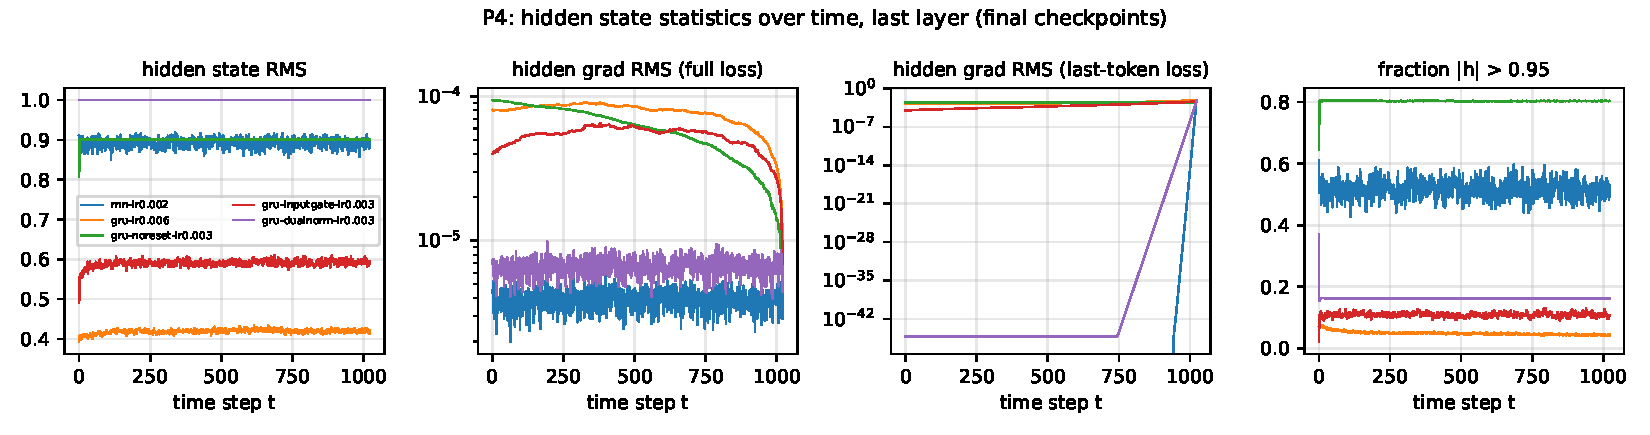
\includegraphics[width=\linewidth]{p4_temporal.pdf}
\caption{P4: last recurrent layer over time for the tanh modern RNN, the GRU and the dual gate cells (final checkpoints).}
\label{fig:p4time}
\end{figure}

\begin{table}[h]\centering\small
\caption{P4 context tests: increase of the last token loss (nats) with $k$ recent tokens; final checkpoints.}
\label{tab:p4ctx}
\begin{tabular}{llrrrrr}\toprule
model & first token & $k=1$ & 4 & 16 & 64 & 256\\\midrule
tanh modern RNN & dropped & 42.3 & 54.9 & 56.1 & 49.1 & 39.3\\
tanh modern RNN & restored & 1.91 & 0.50 & 0.16 & 0.00 & 0.00\\
GRU ($\lr$=0.006) & dropped & 2.57 & 0.85 & 0.28 & 0.13 & 0.01\\
GRU ($\lr$=0.006) & restored & 2.11 & 0.75 & 0.17 & 0.11 & 0.01\\
dual gate, normalised & dropped & 263 & 82.3 & 4.94 & 0.59 & 6.52\\
dual gate, normalised & restored & 1.95 & 0.48 & 0.08 & 0.04 & 0.00\\
\bottomrule\end{tabular}
\end{table}
